\section{Background and Motivation}\label{sec:background}

\begin{figure*}[t]
	\centering
	
	\subfloat[short for lof][Routing state before reconfiguration.] {
		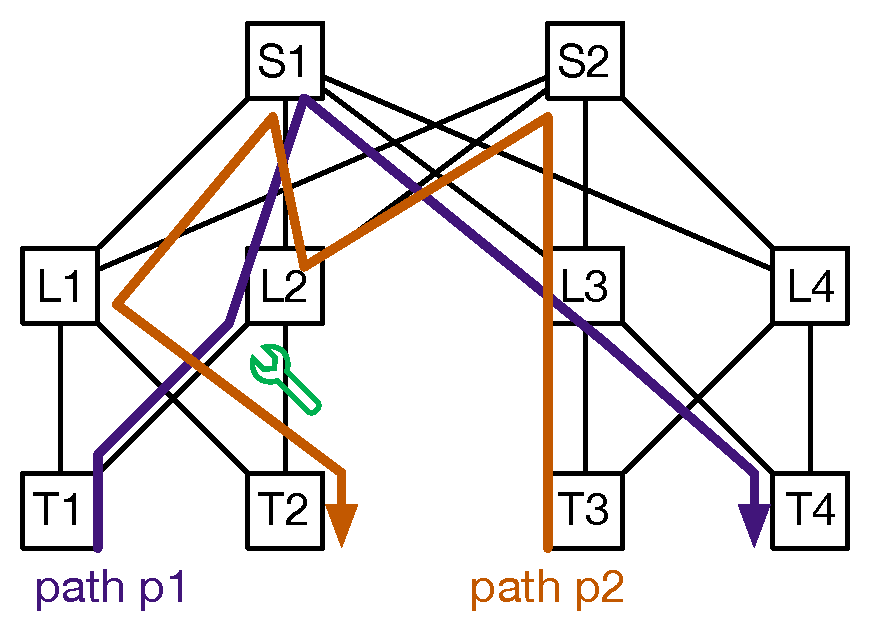
\includegraphics[width=0.33\textwidth] {figs/deadlock_tree_a}
	}
	\subfloat[short for lof][Routing state after reconfiguration.]{
		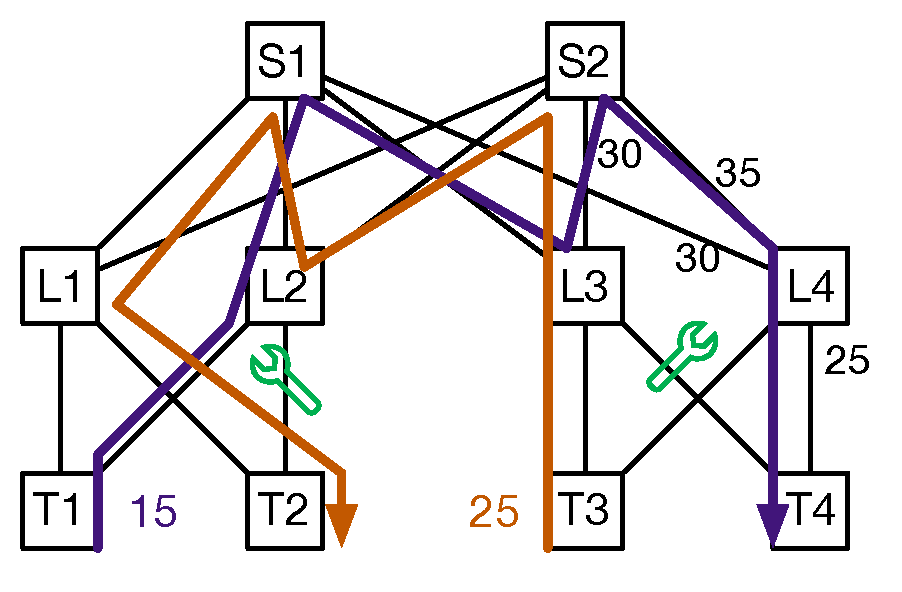
\includegraphics[width=0.33\textwidth] {figs/deadlock_tree_b}
	}
%	\subfloat[short for lof][Traffic among switches L2, L3, S1 and S2.]{
%		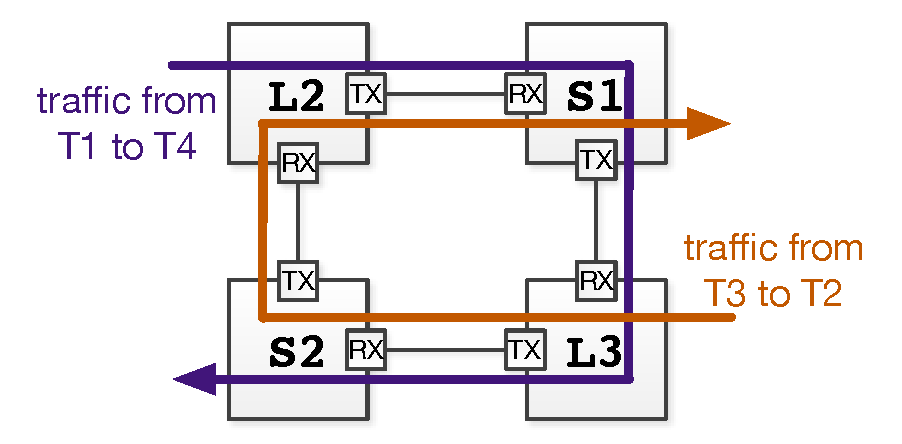
\includegraphics[width=0.3\textwidth] {figs/deadlock_tree_c}
%	}
	\subfloat[short for lof][Buffer dependencies among ingress queues.] {
		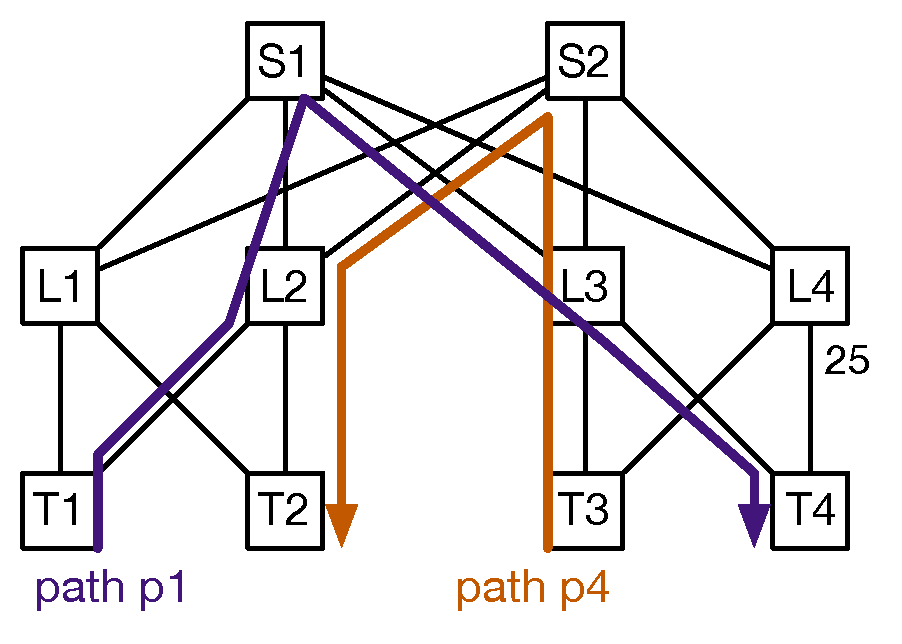
\includegraphics[width=0.25\textwidth] {figs/deadlock_tree_d}
	}
	
	\caption{Reconfiguration-induced deadlock case for leaf-spine topology.}\label{fig:treecase}
	
\end{figure*}

\subsection{PFC Deadlock Problem}\label{subsec:pfcdeadlock}


\textbf{Priority-based Flow Control (PFC)}: The deployment of RDMA over Ethernet requires PFC  to provide a lossless L2 network. PFC is a mechanism for ensuring zero packet loss under congestion in data center bridging (DCB) networks. PFC allows an overwhelmed network device to send a PAUSE frame to its immediate upstream device, which halts the transmission of the sender for a specified period of time.  

PFC works in a per ingress queue fashion. When PFC is enabled, the switch will maintain a counter to track the virtual queue length of each ingress queue. Once the queue length exceeds a pre-configured PFC threshold, a PAUSE frame will be generated.

\textbf{PFC deadlock problem:} The using of PFC can cause deadlock problem. Deadlock may arise when there is cyclic buffer dependency in the network. Once a PFC deadlock is created, a set of ingress queues form a permenant pause cycle, and no packet is allowed to be transmitted inside the cycle.


\subsection{Reconfiguration-induced Deadlock}\label{subsec:reconfigdeadlock}

PFC deadlock can be avoided by leveraging a routing function that introduces no cycle in the buffer dependency graph. However, this approach cannot eliminate the cyclic buffer dependency during routing reconfiguration.

In this part, we use examples to show 1) cyclic buffer dependency can be generated for both tree based and non-tree based DCNs when the routing reconfiguration is not well planed; 2) a bad deadlock-free reconfiguration plan will lead to a slow reconfiguration process.

\subsubsection{Deadlock Under Tree Based DCNs}\label{subsubsec:treecase}
\begin{figure*}[t]
	\centering
	
	\subfloat[short for lof][A 4-node network \textbf{N}.] {
		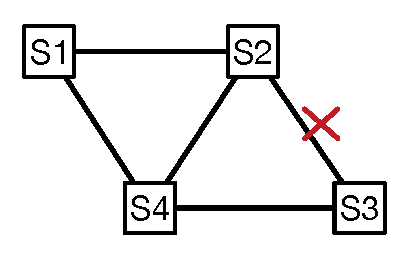
\includegraphics[width=0.3\textwidth] {figs/deadlock_nontree_a}
	}
	\subfloat[short for lof][Routing spanning tree \textbf{T1}.]{
		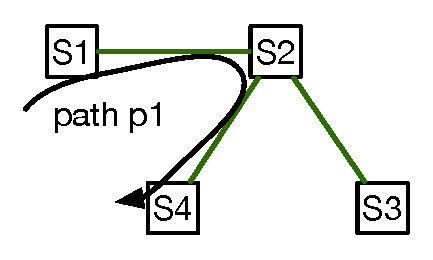
\includegraphics[width=0.3\textwidth] {figs/deadlock_nontree_b}
	}
	\subfloat[short for lof][Routing spanning tree \textbf{T2}.]{
		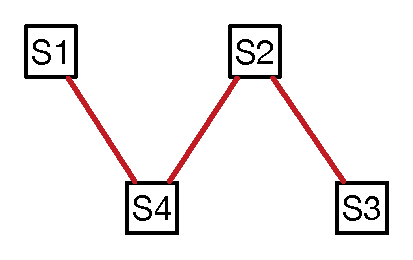
\includegraphics[width=0.3\textwidth] {figs/deadlock_nontree_c}
	}
	
	\subfloat[short for lof][Routing spanning tree \textbf{T3}.] {
		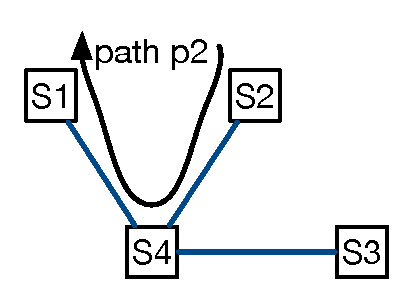
\includegraphics[width=0.3\textwidth] {figs/deadlock_nontree_d}
	}
	\subfloat[short for lof][Routing spanning tree \textbf{T4}.] {
		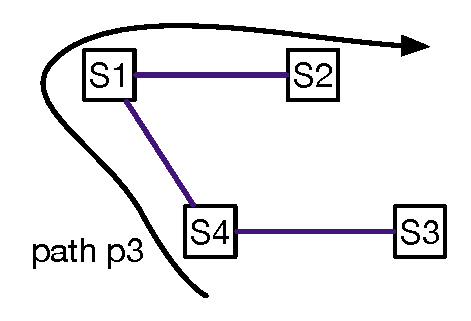
\includegraphics[width=0.3\textwidth] {figs/deadlock_nontree_e}
	}
	\subfloat[short for lof][Buffer dependency graph.]{
		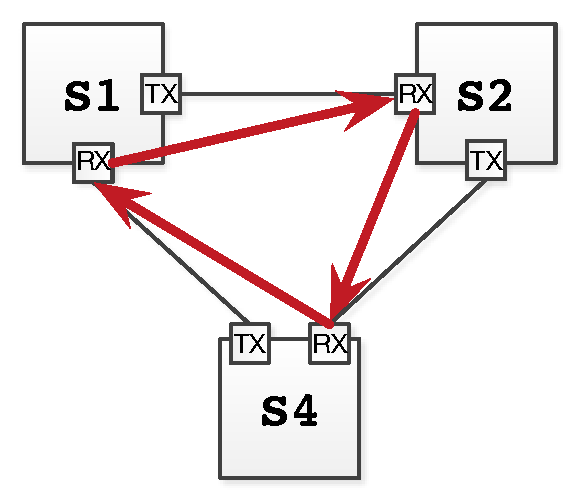
\includegraphics[width=0.3\textwidth] {figs/deadlock_nontree_f}
	}
	
	\caption{Reconfiguration-induced deadlock case for non-tree topology.}\label{fig:nontreecase}
	
\end{figure*}

Fig.~\ref{fig:treecase}(a) shows a small Leaf-Spine DCNs. The capacity of all the links are 40Gbps. Due to maintenance issue, the network operator now wants to replace two links L2-T2 and L3-T3 in the topology. To avoid long-term packet loss during link replacement, the network traffic passing through these two links needs to be migrated to some other paths. 

In this example, we consider the migration of the traffic from switch T1 to switch T4 following the path T1-L2-S1-L3-T4, and the traffic from switch T3 to switch T2 following the path T3-L3-S2-L2-T2. 

There are three alternative paths that the traffic from T1 to T4 can migrate to: 1) \textit{path-1} along T1-L1-S1-L4-T4; 2) \textit{path-2} along T1-L2-S1-L4-T4; 3) non-shortest \textit{path-3} along T1-L2-S1-L3-S2-L4-T4. As we can find in Fig.~\ref{fig:treecase}(a), the traffic load from T1 to T4 is 15Gbps. \textit{Path-1} and \textit{path-2} are not congestion-free choices as the load on link S1-L4 are 30Gbps, larger than 25Gbps. \textit{Path-3} is a congestion-free choice as the load on links L3-S2, S2-L4 and L4-T4 are all smaller than 25Gbps. 

While not explicitly drawn in the Fig.~\ref{fig:treecase}(a), non-shortest path T3-L3-S2-L2-S1-L1-T2 is also the only congestion-free choice that the traffic from T3 to T2 can migrate to. Fig.~\ref{fig:treecase}(b) shows the routing state after migrating the traffic to the two non-shortest paths. 

In Fig.~\ref{fig:treecase}(c), we focus on the buffer dependency among four switches L2, L3, S1 and S2. We reposit the locations of these four switches and draw both ingress queues (RX) and egress queues (TX) for the purpose of better explanation. The buffer dependency introduced by the two non-shortest paths in Fig.~\ref{fig:treecase}(b) are drawn with directed lines. As we can see, there is a cyclic buffer dependency among the ingress queues. This indicates that the network is now exposed to the danger of PFC deadlock.

To avoid possible PFC deadlock problem, one safe congestion-free reconfiguration plan is to replace the two links one by one. Only using one non-shortest path will not introduce cyclic buffer dependency into the network.



\subsubsection{Deadlock Under Non-tree Based DCNs}\label{subsubsec:nontreecase}



\begin{figure}[t]
	\centering
	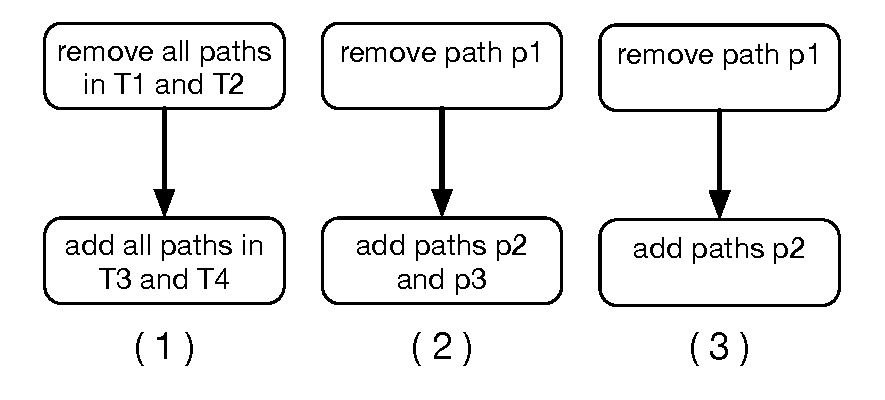
\includegraphics[width=0.45\textwidth] {figs/dfschemes}
	\caption{Three deadlock-free reconfiguration schemes.}\label{fig:dfschemes}
	
\end{figure}

As shown in Fig.~\ref{fig:nontreecase}(a), in this example we consider a 4-node network \textbf{N}. This topology can be a subgraph of many non-tree based DCNs, like HyperX, Jellyfish and BCube.

Fig.~\ref{fig:nontreecase}(b)-(e) are four spanning trees \textbf{T1}-\textbf{T4} which specify the routing paths that can be used in \textbf{N}. For example, path p1 is a legal routing path specified in \textbf{T1}.  

Let $\textbf{R}_i$ be the set of paths specified in tree \textbf{Ti}. Let $\textbf{R}_s = \textbf{R}_1 \cup \textbf{R}_2$, and $\textbf{R}_t = \textbf{R}_3 \cup \textbf{R}_4$. It is easy to check both $\textbf{R}_s$ and $\textbf{R}_t$ are deadlock-free routing functions. Initially,  $\textbf{R}_s$ are used as the routing function of \textbf{N}. Due to the failure of link S2-S3, switch S3 becomes unreachable. To maintain the connectivity of \textbf{N}, we can perform a routing reconfiguration to transition from $\textbf{R}_s$ to $\textbf{R}_t$.

During the reconfiguration process, if path p2 in \textbf{T3} and path p3 in \textbf{T4} are added to the routing function before path p1 in \textbf{T1} is removed, a cyclic buffer dependency will be generated, as shown in Fig.~\ref{fig:nontreecase}(f). This may cause a PFC deadlock as we explained in Sec.~\ref{subsec:pfcdeadlock}.

In Fig.~\ref{fig:dfschemes}, we present three possible deadlock-free reconfiguration schmes. The first scheme is to remove all the paths in \textbf{T1} and \textbf{T2} before adding any new paths in \textbf{T3} and \textbf{T4}. This scheme will lead to a slow reconfiguration process as all the operations of adding new paths are delayed by the operations of removing old paths. 

The second scheme only requires path p1 is removed before paths p2 and p3 are added. All the other paths not mentioned can be updated freely without any order constraint. Hence the speed of routing reconfiguration can be improved. The third scheme is an optimized reconfiguration scheme in terms of imposing minimum order constraints on the update actions. The intuition here is that as long as paths p1, p2 and p3 do not take effect at the same, deadlock-free can be well guaranteed. 

While for this example it may seem easy to find a deadlock-free reconfiguration scheme that requires minimum order constraints, in general it is difficult as there are combinatorial such schemes to be checked.


\subsection{Measurement of Rule Update Time}\label{subsec:updatetime}

In this part, we demonstrate that adding order constraints to the update of switch rules will significantly prolong the reconfiguration process.








%In Fig.~\ref{fig:deadlock_case}, we use a simple example to show how  deadlock can be created when there is a cyclic buffer dependency among a set of switch buffers.
%
%\begin{figure}[t]
%	\centering
%	
%	\subfloat[short for lof][Topology and flows.] {
%		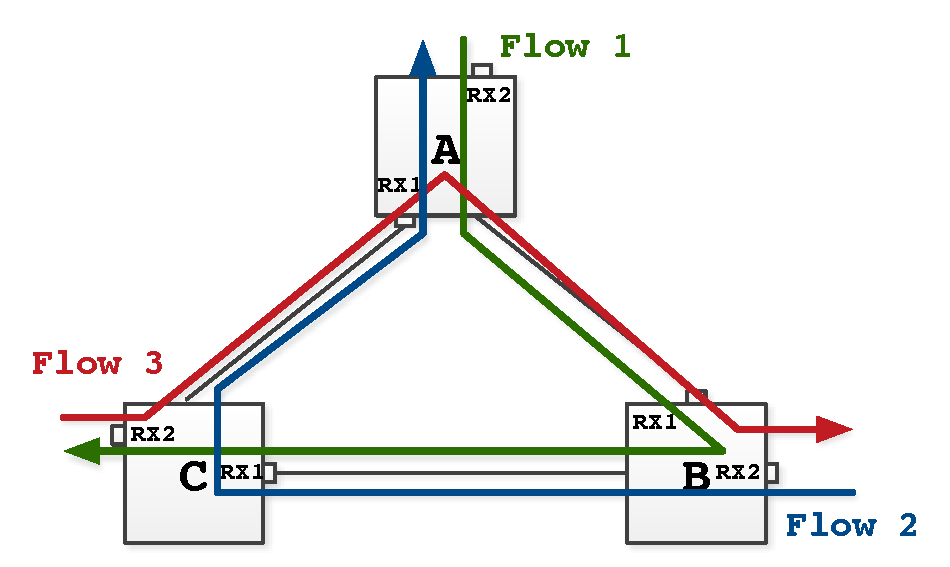
\includegraphics[width=0.3\textwidth] {figs/case1_topo}
%	}
%	\subfloat[short for lof][Buffer dependency graph.]{
%		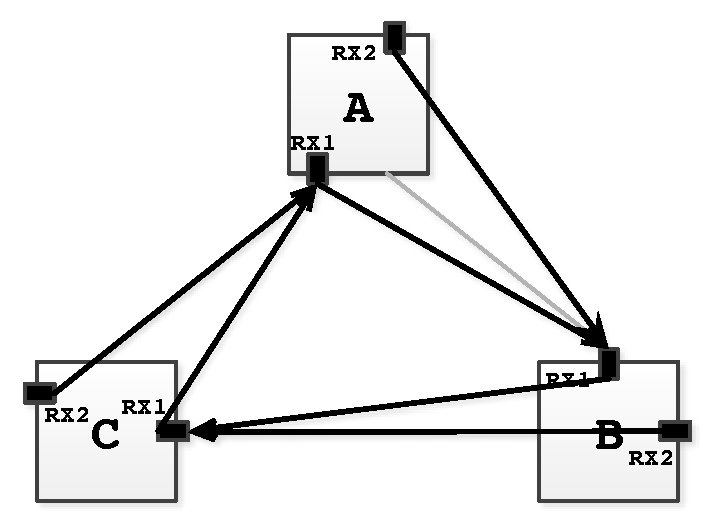
\includegraphics[width=0.2\textwidth] {figs/case1_dependency}
%	}
%	
%	\caption{Flows 1, 2 and 3 forms a cycle in the buffer dependency graph that can create a routing deadlock. In both figures, RX represents an ingress switch queue.}\label{fig:deadlock_case}

%\end{figure}
%
%As shown in Fig.~\ref{fig:deadlock_case}(a), three flows are runing over three switches A, B and C. Flow 1 starts at a host (not shown) attached to A, passes through B, and ends at a host attached to C. Flow 2 and flow 3 are two symmetric flows of flow 1. Buffer dependencies among active ingress queues are drawn in Fig.~\ref{fig:deadlock_case}(b). The path flow 1 takes introduces two dependency links, one from RX2 of A to RX1 of B, the other from RX1 of B to RX1 of C. Similarly, paths taken by flow 2 and flow 3 introduce the other four dependency links in Fig.~\ref{fig:deadlock_case}(b).

%As we can find in Fig.~\ref{fig:deadlock_case}(b), the paths taken by the 3 flows introduce a cyclic buffer dependency among switches A, B and C. When network congestion occurs, it is possible that all the three RX1 queues become full of the packets destined for the next-hop switch and trigger PFC PAUSE simultaneously. Then a PFC deadlock is created as links A-B, B-C and C-A will be permanently paused and no packet in the three RX1 queues can ever get drained.
